%!TEX TS-program = xelatex
%!TEX root = ../../maxwell2018thesis.tex

\begin{preamble}[Presentational Conventions]
\phantomsection
\addcontentsline{toc}{part}{Presentational Conventions}

A number of different presentational conventions have been employed in this thesis. These are listed below for reference.

\glsunset{acr:url}

\begin{itemize}
    
    \item{Spelling is according to the \emph{Oxford English Dictionary}; the version referred to is searchable online at \url{https://en.oxforddictionaries.com/}.}
    
    \item{\emph{Italicised text} is used to define a term, but not thereafter. This applies to acronyms, where the full expansion is presented initially; associated abbreviations are used thereafter. Full expansions of an acronym may be reused if required.}
    
    \item{\darkblueboxbold{Research questions} and descriptions for \blueboxbold{terms} and \blueboxbold{components} used in this research are presented inline within shaded boxes.}
    
    \begin{itemize}
        
        \item{We also refer to a number of different \emph{stopping strategies} throughout this thesis, each with their own name and a variable. We use the notation \stoppingstratbox{Name}{Value} to present these strategies.}
        
    \end{itemize}
    
    \item{\glsplural{acr:url} are used to provide references for claims and to refer readers to external resources. As these resources may become unavailable over time, the date of \textbf{L}ast \textbf{A}ccess follows each~\gls{acr:url} -- e.g. \url{http://www.dmax.org.uk}\urlaccessed{2018-06-07}.}
    
    \item{Pseudo-code that is presented within this thesis uses the \emph{HAGGIS} high-level reference programming language, as per~\cite{cutts2014haggis}.}
    
    \item{Plots use a consistent colour scheme across chapters to maximise understandability. Colours employed are based upon colour schemes as used in the online tool outlined by~\cite{harrower2003colorbrewer}.}
    
    \item{Cell \darkbluebox{highlighting} is used throughout the tables within this thesis to represent values of interest -- whether they simply are the best reported, or illustrate a significant difference. Refer to the caption of each table for the specific meaning of what highlighting denotes for said table.}
    
\end{itemize}

\glsreset{acr:url}

% While all figures are specially created for use in this thesis, several diagrams are based upon the figures provided in other publications. Where this is the case, acknowledgement of the source publication is included in the relevant figure caption. Permission was sought to include these figures wherever possible. Several vector artwork images have also been procured from \texttt{freepik.com} for non-commercial use.

The main body of this thesis is typeset in 12 point Palatino (body) with 1\sfrac{1}{2} line spacing. Headers, figures and tables (along with their associated captions) use \headerfont\selectfont Foundry Sterling\normalfont\selectfont. The names of tools used and other minor components of this thesis (e.g. table grouping headers) are also represented using \headerfont\selectfont Foundry Sterling\normalfont\selectfont. For example, fictional retrieval system \searchlogo~is used to demonstrate various concepts throughout this work.\footnote{Any resemblance of \searchlogo~to real-world retrieval systems is unintentional and purely coincidental.}

This thesis is typeset using \XeTeX\ version \texttt{0.99998}. A custom \TeX\ class (\texttt{.cls}) has been developed and used for typesetting. The class is largely in compliance with University of Glasgow PhD thesis regulations.

Illustrations are used extensively throughout this thesis to better demonstrate points and concepts being conveyed. While the author of this thesis drew a majority of the illustrations in \emph{Adobe \textregistered~Illustrator \textregistered~CS6,} a number of free, pre-made vector artworks have been downloaded from \emph{freepik.com} and incorporated within this thesis. This statement therefore serves as acknowledgement that these artworks have been used and are included on the assumption that no part of this work will be used for commercial purposes.

In addition to the points described above, \blueboxbold{flowcharts} are also extensively used in this thesis to demonstrate the conceptual models that we outline. A standard design for flowcharts is employed, and follows the design guidelines as outlined in \href{https://www.iso.org/standard/11955.html}{\texttt{ISO 5807:1985}}\footnote{\href{https://www.iso.org/standard/11955.html}{\texttt{ISO 5807:1985}} defines symbols to be used in information processing documentation and gives guidance on conventions for their use in data flowcharts, program flowcharts, system flowcharts, program network charts, system resources charts.}. Other models presented in the literature also employ such an approach (e.g.~\cite{thomas2014modelling_behaviour}). The following example demonstrates the symbols used in this thesis.

\begin{figure*}[h!]
    \centering
    \resizebox{1\hsize}{!}{
    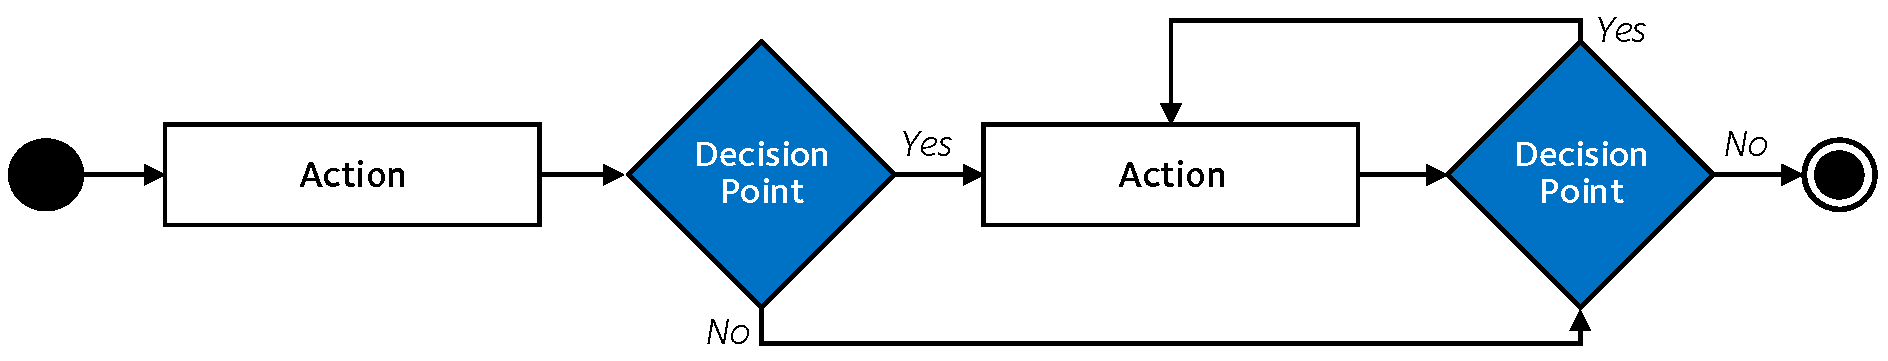
\includegraphics{figures/ch0-example.pdf}}
\end{figure*}

Note that the sequence of events begins with a~
\includegraphics[height=\fontcharht\font`\d]{figures/ch0-example-start.pdf}, and ends at a~
\includegraphics[height=\fontcharht\font`\d]{figures/ch0-example-end.pdf}.\footnote{Note that these symbols are not part of the \href{https://www.iso.org/standard/11955.html}{\texttt{ISO 5807:1985}} standard; they are part of the \emph{Unified Modelling Language (UML)} specification, and have been included to ensure diagrams are simple to understand.} Diagram flow can be deduced by examining the direction of arrows. Actions (or events) are denoted by the text contained within unfilled rectangles~
\includegraphics[height=\fontcharht\font`\d]{figures/ch0-example-action.pdf}, with decision points represented as~
\includegraphics[height=\fontcharht\font`\d]{figures/ch0-example-decision.pdf}. The different outcomes of decisions are denoted by the \emph{italicised} text at each output point of a~
\includegraphics[height=\fontcharht\font`\d]{figures/ch0-example-decision.pdf}.

\end{preamble}